\documentclass[11pt,a4paper]{article}
\usepackage[spanish,es-nodecimaldot]{babel}
\usepackage[T1]{fontenc}
\usepackage[utf8]{inputenc}
\usepackage{helvet,courier,microtype,graphicx,booktabs,tabularx,array,enumitem}
\renewcommand{\familydefault}{\sfdefault}
\usepackage[margin=2cm,headheight=20pt,footskip=26pt]{geometry}
\usepackage[table]{xcolor}
\usepackage[most]{tcolorbox}
\usepackage{fancyhdr,hyperref}
\ifdefined\pdfinfoomitdate\pdfinfoomitdate=1\fi
\ifdefined\pdftrailerid\pdftrailerid{}\fi
\ifdefined\pdfsuppressptexinfo\pdfsuppressptexinfo=15\fi
\definecolor{navy}{HTML}{17324D}
\definecolor{teal}{HTML}{087E83}
\definecolor{muted}{HTML}{536678}
\definecolor{pale}{HTML}{EEF7F8}
\hypersetup{colorlinks=true,urlcolor=teal,linkcolor=teal,pdftitle={Adenda de operación BI e IA - 25 de noviembre de 2026},pdfauthor={Proyecto académico BI}}
\pagestyle{fancy}\fancyhf{}
\fancyhead[L]{\small\color{teal}\textbf{BI + IA\enspace /\enspace GUÍA DE OPERACIÓN}}
\fancyhead[R]{\small\color{muted}Adenda de noviembre de 2026}
\fancyfoot[L]{\footnotesize\color{muted}Prototipo académico · Operación supervisada}
\fancyfoot[R]{\footnotesize\thepage\ / 7}
\renewcommand{\headrulewidth}{0.4pt}
\setlength{\parindent}{0pt}\setlength{\parskip}{6pt}
\setlist[enumerate]{leftmargin=*,itemsep=4pt,topsep=4pt}
\setlist[itemize]{leftmargin=*,itemsep=3pt,topsep=3pt}
\renewcommand{\arraystretch}{1.2}
\newcolumntype{Y}{>{\raggedright\arraybackslash}X}
\newtcolorbox{nota}[1][]{colback=pale,colframe=teal!35,boxrule=.5pt,arc=2mm,left=3mm,right=3mm,top=2mm,bottom=2mm,#1}
\newcommand{\titulo}[2]{\vspace*{2mm}{\small\color{teal}\textbf{#1}}\par{\LARGE\color{navy}\textbf{#2}}\par\vspace{3mm}}
\newcommand{\subtitulo}[1]{\par\vspace{2mm}{\large\color{navy}\textbf{#1}}\par}
\begin{document}
\titulo{ACTUALIZACIÓN OPERATIVA · 25 DE NOVIEMBRE DE 2026}{Continuar el trabajo y usar OpenAI}
Esta adenda acompaña al manual principal. Explica los cambios de navegación,
sesión, catálogo y proveedor de IA para que las programadoras y los usuarios
puedan repetir el recorrido sin perder su contexto.

\begin{nota}
\textbf{La idea central.} La IA interpreta y propone. La aplicación comprueba
referencias y reglas; una persona revisa las decisiones. Sólo después se prepara
y confirma el ETL. Un resultado de IA, por sí solo, no acredita ventas correctas.
\end{nota}

\subtitulo{Seis conceptos para empezar}
\begin{tabularx}{\linewidth}{@{}p{3.1cm}Y@{}}
\toprule\textbf{Concepto}&\textbf{Qué significa en esta herramienta}\\\midrule
Proveedor\newline y modelo & El proveedor ofrece el servicio; el modelo procesa la solicitud.
OpenAI y Groq son proveedores distintos, aunque algunas API se parezcan.\\
Metadatos & Nombres de tablas y columnas, tipos, claves y relaciones.
Describen la estructura; no son las filas de las ventas.\\
Viabilidad & Revisión previa del respaldo de una necesidad. Puede señalar datos
directos, derivaciones y límites por resolver.\\
Propuesta BI & Modelo dimensional, medidas, indicadores y plan de transformación
que aún deben revisarse y aprobarse.\\
ETL & Extracción, transformación y carga de los datos en el datamart.
Su ejecución es una acción separada de aprobar la propuesta.\\
Conciliación & Contraste de cantidades e importes equivalentes entre origen y
destino. Debe corresponder a la misma fuente y ejecución.\\\bottomrule
\end{tabularx}

\subtitulo{Quién hace cada parte}
La \textbf{administración} configura conexiones, credenciales, modelos y permisos.
El \textbf{analista BI} expresa la necesidad, revisa el significado comercial,
aprueba la propuesta y confirma el ETL autorizado.
La \textbf{gerencia} consulta indicadores y hace preguntas sobre los resultados.
Las opciones visibles dependen de los permisos asignados.

\subtitulo{Orden de trabajo}
\textbf{Fuente y metadatos} $\rightarrow$ \textbf{Catálogo} $\rightarrow$
\textbf{Necesidad y viabilidad} $\rightarrow$ \textbf{Propuesta y aprobación}
$\rightarrow$ \textbf{ETL y conciliación} $\rightarrow$ \textbf{Análisis}.

La misma lógica se aplica a AdventureWorks y WideWorldImporters. Cambiar la
fuente cambia el contexto de trabajo; no une las bases ni autoriza sus resultados
como si fueran un único negocio. Otros motores requieren sus adaptadores.

\newpage
\titulo{01 · NAVEGACIÓN Y SESIÓN}{Volver al lugar correcto}
\subtitulo{Recargar y usar el botón Atrás}
\begin{enumerate}
\item Entre en un módulo desde la barra lateral. Si recarga el navegador,
la aplicación recupera el módulo de esa pestaña cuando la cuenta conserva acceso.
\item Desde \textbf{Inicio}, abra \textbf{Revisar configuración}.
Avance hasta el paso que desee revisar y pulse \textbf{Revisar este paso}.
En el módulo de destino aparecerá \textbf{Atrás}.
\item Pulse \textbf{Atrás} para regresar a Inicio y al paso de preparación
desde el cual salió. En el paso 5, \textbf{Elegir datamart} conserva ese mismo retorno.
\item Si entra mediante \textbf{Crear propuesta de datamart} desde Inicio,
\textbf{Atrás} permite volver a ese origen. Si entra directamente por la barra
lateral, no se añade un retorno guiado.
\item En \textbf{Analítica de ventas}, \textbf{Consultar respaldo} abre el espacio
del datamart. Su \textbf{Atrás} vuelve al análisis. Cada fuente conserva su selección confirmada, incluso una ejecución anterior,
con indicador, filtros y vista. Restablecer afecta sólo esa fuente; el chat no se guarda.
\end{enumerate}

\subtitulo{Configurar el tiempo de sesión}
\begin{minipage}[t]{0.56\linewidth}
En \textbf{Parámetros}, una persona autorizada puede editar
\textbf{Duración de la sesión (minutos)}. El valor inicial es \textbf{60 minutos}; el rango permitido va de
\textbf{15 a 240 minutos}. Para ensayos largos puede elegir 60 o 120 minutos.

El plazo cuenta desde el inicio de sesión: usar botones no reinicia el contador.
Un cambio de duración afecta a los próximos inicios, no extiende tokens ya emitidos.
\begin{enumerate}
\item Antes de un ensayo nuevo, ajuste y guarde el tiempo en Parámetros.
Inicie otra sesión para recibir la nueva duración.
\item Si vence la sesión durante el trabajo, autentíquese de nuevo y compruebe
la fuente, el punto recuperado y las preguntas de la necesidad.
\item Autorice otra vez el destino de IA cuando se solicite y repita la viabilidad
antes de generar.
\end{enumerate}
El cierre voluntario limpia el borrador local. Si ya tiene un borrador en curso,
considere ese efecto antes de cerrar sesión para aplicar un nuevo tiempo.
No recargue una operación larga para intentar ejecutarla otra vez.
\end{minipage}\hfill
\begin{minipage}[t]{0.39\linewidth}
\vspace{0pt}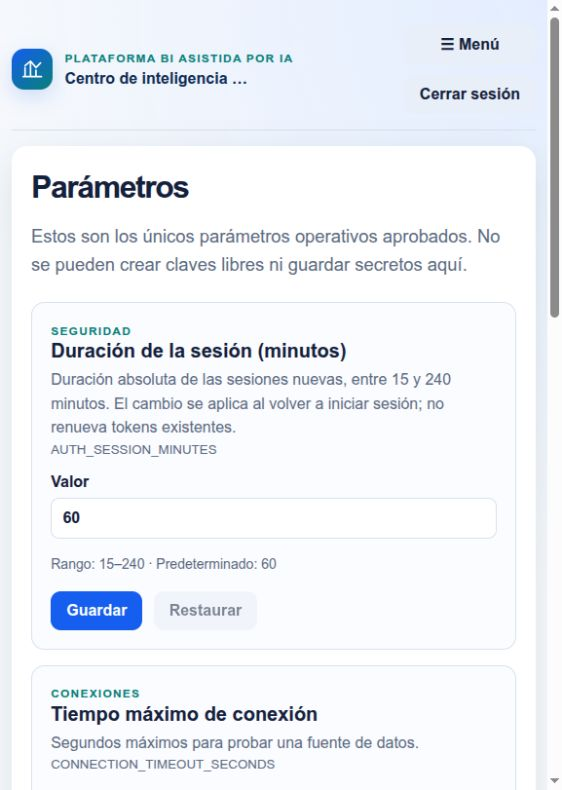
\includegraphics[width=\linewidth]{recursos/parametros-sesion-60.jpg}
{\footnotesize\color{muted}Captura real del 25 de noviembre. El parámetro muestra
60 minutos y explica el rango y la aplicación al próximo inicio de sesión.}
\end{minipage}

\begin{nota}
\textbf{Si la ejecución guardada ya no está disponible,} la aplicación debe
informarlo. Use la acción explícita para restablecer la selección y elegir otro
expediente; no interprete otra ejecución como si fuera la anterior.
\end{nota}

\newpage
\titulo{02 · ADMINISTRACIÓN}{Configurar OpenAI paso a paso}
Se necesita una API key válida, acceso al modelo y crédito o facturación
disponible en el proyecto de OpenAI. La aplicación no puede deducir esos permisos
por la suscripción de ChatGPT: se comprueban al probar la conexión.

\begin{enumerate}
\item Abra \textbf{Preparación del entorno > Configuración LLM} con una cuenta
que tenga permiso para administrar esta opción.
\item En \textbf{Crear configuración LLM}, escriba un nombre que pueda reconocer,
por ejemplo, \textit{OpenAI para demostración BI}.
\item Seleccione \textbf{OpenAI}. Revise los valores sugeridos de la tabla.
El identificador del modelo es editable si su proyecto utiliza otro compatible.
\item Guarde la configuración. Después, en su registro, elija
\textbf{Registrar credencial}. Escriba la API key directamente en ese campo privado.
\item Confirme el registro. El sistema conserva la clave cifrada y muestra su
estado; no necesita volver a mostrar el valor para poder utilizarlo.
\item Pulse \textbf{Probar conexión}. La prueba envía una solicitud técnica pequeña,
sin metadatos de sus bases ni filas comerciales. Puede consumir tokens de API.
\item Si la comprobación es correcta, pulse \textbf{Activar} en la configuración.
Sólo hay un proveedor activo para las operaciones de IA de la aplicación.
\item Vuelva a Inicio o al Asistente y compruebe el proveedor y modelo visibles.
Autorice el envío de metadatos al destino que realmente haya elegido.
\end{enumerate}

\begin{tabularx}{\linewidth}{@{}p{4.4cm}Y@{}}
\toprule\textbf{Campo}&\textbf{Valor inicial recomendado}\\\midrule
Proveedor & OpenAI\\
URL del servicio & \url{https://api.openai.com/v1}\\
Modelo económico & \texttt{gpt-6-luna}\\
Nivel de razonamiento & Bajo\\\bottomrule
\end{tabularx}

\newpage
\titulo{03 · MODELOS Y COSTOS}{Elegir cómo utilizar el crédito}
\subtitulo{Presupuesto y evidencia son criterios distintos}
Luna admite Responses y salidas estructuradas; se recomienda con razonamiento
bajo para controlar el costo. Sol, con razonamiento medio, tiene recorridos
completos comprobados en ambas bases. Luna sólo pasó una prueba técnica de conexión
y JSON estructurado; no se ensayaron viabilidad, propuesta ni ETL con él.

{\small\begin{tabularx}{\linewidth}{@{}p{3cm}rrrY@{}}
\toprule\textbf{Modelo}&\textbf{Entrada}&\textbf{Salida}&\textbf{Ejemplo}&\textbf{Evidencia aquí}\\\midrule
GPT-6 Luna & 0,10 & 0,50 & 0,0020 & Conexión + JSON; bajo\\
GPT-5.4 mini & 0,75 & 4,50 & 0,0165 & No ensayado\\
GPT-6.1 Terra & 1,00 & 5,00 & 0,0200 & No ensayado\\
GPT-6.2 Sol & 2,00 & 10,00 & 0,0400 & Flujo completo; medio\\
GPT-6.2 Astra & 8,00 & 40,00 & 0,1600 & No ensayado; costo alto\\\bottomrule
\end{tabularx}}
{\footnotesize Importes en USD. Entrada y salida: tarifas Standard por millón de
tokens, contexto corto, al 25 de noviembre. Ejemplo estimado: 10000 tokens de
entrada y 2000 de salida, sin caché ni razonamiento adicional, reintentos u otros
cargos. Las tarifas de Luna son un 95\% menores; eso no garantiza igual ahorro por respuesta.}

Sol se usó en AdventureWorks (propuesta 136, ejecución 24) y WideWorldImporters
(135, 23). No se conservaron costos facturados por solicitud: una variación del
saldo no se puede atribuir íntegramente a esas pruebas sin revisar el registro de OpenAI.

\subtitulo{Crédito, razonamiento y consumo}
El límite de salida incluye razonamiento interno y JSON: 4096 tokens para
automático, mínimo o bajo; 8192 para medio y 16384 para alto. Un presupuesto mayor
se respeta hasta 32768. Son \textbf{límites por solicitud}, no un cobro completo
obligatorio; un flujo puede realizar varias solicitudes.

\textbf{Groq tiene otra cuenta y cuota.} Sus modelos no consumen los créditos de
OpenAI. Use cada clave exclusivamente con el proveedor al que pertenece.

\subtitulo{Una rutina sencilla para gastar con criterio}
\begin{enumerate}
\item Empiece con \textbf{Luna y razonamiento bajo} si prioriza el presupuesto.
Revise el resultado antes de repetir una llamada; no suba a Sol automáticamente.
\item Confirme fuente, objetivo y preguntas antes de solicitar IA. Un cambio
posterior de alcance puede exigir otra revisión.
\item Para sustentar, abra propuestas aprobadas, expedientes y paneles ya
publicados. Consultarlos no obliga a generar otra propuesta ni otro ETL con IA.
\item Solicitar sugerencias, viabilidad, propuestas o conversación puede consumir
API. Realice sólo la operación que quiera demostrar y consulte el gasto en OpenAI.
\end{enumerate}

\newpage
\titulo{04 · CATÁLOGO Y ASISTENTE}{Resolver preguntas que ya no están}
Un borrador puede conservar preguntas retiradas o sin respaldo en el catálogo.
En la captura de WideWorldImporters, esa selección antigua provocó un bloqueo
antes de llamar a la IA. Revise la selección vigente de su propia fuente.

\subtitulo{Qué hacer al recuperar un borrador}
\begin{enumerate}
\item Lea el aviso de cambio del catálogo. El objetivo escrito se conserva.
Las preguntas todavía válidas permanecen seleccionadas; las retiradas salen
de la selección del borrador.
\item Compruebe la \textbf{fuente en contexto}. Una pregunta propia de
AdventureWorks no debe aparecer seleccionada en WideWorldImporters por haber
trabajado antes con ella.
\item Revise las preguntas visibles y la periodicidad. Si una pregunta necesaria
ya no existe, revise el catálogo con una persona autorizada. No sustituya su
significado sólo por escoger una etiqueta parecida.
\item Compruebe el proveedor, autorice el envío y pulse \textbf{Validar viabilidad}.
El cambio de alcance invalida la revisión anterior y requiere otra comprobación.
\item Examine el respaldo y los límites. Sólo entonces continúe con la generación
de conceptos y propuesta. No es necesario borrar todas las versiones guardadas.
\end{enumerate}

\subtitulo{Cómo leer el respaldo de una necesidad}
\begin{tabularx}{\linewidth}{@{}p{3cm}Y@{}}
\toprule\textbf{Resultado}&\textbf{Decisión del analista}\\\midrule
Directo & Revise que la referencia encontrada represente el dato comercial pedido.
Que exista una columna no demuestra la calidad de sus valores.\\
Derivable & Compruebe la relación o fórmula candidata. Puede resolverse mediante
las operaciones permitidas, pero aún necesita validación dentro de la propuesta.\\
Ambiguo & Aclare el evento, la fecha, la entidad o la fórmula. Un pedido y una
factura no representan necesariamente el mismo proceso comercial.\\
No disponible & Reduzca el objetivo o incorpore una fuente autorizada con respaldo.
La IA no debe inventar el dato faltante.\\\bottomrule
\end{tabularx}

\subtitulo{Antes de aprobar la propuesta}
Revise el nivel de detalle: una fila por línea no equivale a una fila por pedido
o factura. Compruebe la fecha, las dimensiones, los importes y cada promedio.
Verifique que cada resultado pedido tenga un indicador disponible: una columna
de cantidad, por sí sola, no demuestra que el panel publicará las unidades.
Si solicita documentos distintos,
su identificador debe estar respaldado: contar líneas no cumple esa petición.

\begin{nota}
\textbf{Consultar una versión histórica no debe reescribirla.} Sus preguntas,
decisiones y evidencia se conservan aunque el catálogo actual cambie. Para cambiar
una versión aprobada utilice el recorrido de una nueva versión corregida.
\end{nota}

\newpage
\titulo{05 · PRÁCTICA GUIADA}{Repetir el recorrido con ambas bases}
Estos ejercicios ayudan a aprender el flujo. Debe revisar la evidencia que
efectivamente presente su instalación; no constituyen una promesa de que cualquier
texto o cualquier respuesta del modelo será aceptado.

\begin{nota}
\textbf{Ejercicio A · AdventureWorks}\par
``Analizar mensualmente los importes registrados y las unidades vendidas por
producto, para revisar su evolución y comparar los productos con mayor resultado,
sin atribuir causas ni añadir fuentes externas.''
\end{nota}
\begin{nota}
\textbf{Ejercicio B · WideWorldImporters}\par
``Analizar mensualmente los importes y cantidades de las líneas facturadas por
producto, para comparar su evolución y desempeño, sin suponer una moneda ni una
composición fiscal que los datos no demuestren.''
\end{nota}

\begin{enumerate}
\item \textbf{Preparar.} Seleccione la fuente del ejercicio. Abra el Explorador
y confirme que la instantánea corresponde a esa conexión. Revise las relaciones
y qué tablas representan el evento comercial.
\item \textbf{Configurar la orientación.} Abra el catálogo de la misma fuente.
Compruebe las preguntas habilitadas de evolución temporal y productos.
Seleccione periodicidad mensual; no cambie preguntas de otra fuente.
\item \textbf{Revisar la necesidad.} Pegue o adapte el objetivo, seleccione sólo
las preguntas pertinentes, autorice el proveedor y valide la viabilidad.
Compruebe las referencias y cualquier límite antes de continuar.
\item \textbf{Revisar la propuesta.} Genere conceptos y modelo. Verifique que
se conservan el evento, el detalle de línea, el mes y el producto solicitados.
Si hay un bloqueo, lea la explicación y corrija su causa antes de aprobar.
\item \textbf{Aprobar y cargar.} Con permiso y criterio suficiente, apruebe la
propuesta. Después abra Datamart de ventas, elija esa propuesta, revise los
indicadores, prepare el plan y confirme la ejecución autorizada del ETL.
\item \textbf{Conciliar.} Revise fuente, propuesta y ejecución del expediente.
La diferencia de filas y las comprobaciones numéricas deben corresponder al mismo
recorrido. Resolver etiquetas semánticas no equivale a cambiar los datos originales.
\item \textbf{Analizar.} Entre al panel y confirme el contexto. Pruebe un año,
un territorio si está disponible, ambas vistas y las exportaciones. Pregunte al
copiloto por la evolución y los límites. Repita después con la otra fuente.
\end{enumerate}

\subtitulo{Cómo reconocer un resultado coherente}
El título, fuente, ejecución y alcance comercial deben coincidir. El tablero
y el copiloto deben explicar las mismas unidades y filtros; una asociación no
prueba causalidad. Al cambiar de contexto se descartan conversaciones anteriores.
No se guardan como resultado confirmado filtros cuya consulta falló o sigue pendiente.

\newpage
\titulo{06 · RESOLUCIÓN DE PROBLEMAS}{Interpretar un aviso y actuar}
\small
\begin{tabularx}{\linewidth}{@{}>{\raggedright\arraybackslash}p{4cm}Y@{}}
\toprule\textbf{Qué observa}&\textbf{Qué debe hacer}\\\midrule
La sesión venció & Autentíquese y revise el punto recuperado. Su duración se configura
en Parámetros y no se reinicia con actividad.\\
No aparece Atrás & Compruebe cómo entró. El retorno contextual corresponde a los
recorridos guiados; la entrada directa por menú mantiene la navegación normal.\\
El catálogo cambió & Revise preguntas y periodicidad; autorice el destino y valide
otra vez. No elimine propuestas ni expedientes para resolver un borrador.\\
OpenAI rechaza la clave & Revise o reemplace la credencial desde su campo privado.
No comparta la clave mediante capturas, documentos o registros.\\
Modelo sin acceso o saldo agotado & Compruebe modelo, proyecto, crédito y permisos
en OpenAI. Agotar crédito no se resuelve repitiendo continuamente la misma llamada.\\
Salida incompleta o contrato inválido & Lea el aviso. La respuesta se descarta;
revise la complejidad, el razonamiento y la configuración. No apruebe un resultado
incompleto ni cambie de proveedor sin revisar el destino.\\
Propuesta con bloqueos & Contraste la necesidad con referencias, evento y fórmulas.
Corregir una petición no significa ocultarla para que el control la acepte.\\
Datos o contexto diferentes & Deténgase y compare fuente, ejecución, propuesta,
filtros y unidad. Consulte el respaldo antes de presentar una conclusión.\\
Consulta pendiente al cambiar filtros & Espere la nueva confirmación. La respuesta
de un chat anterior no se incorpora al contexto nuevo; no se reutiliza como evidencia.\\\bottomrule
\end{tabularx}
\normalsize

\subtitulo{Qué se corrigió en la generación}
El tratamiento de la propuesta conserva todos los requisitos revisados, sin un
recorte que podía omitir los últimos. También distingue un identificador de factura
de una medida monetaria y evita excluir una referencia documental necesaria sólo
por su nombre. Son controles generales: no dependen del nombre de una base.

\textbf{Para las programadoras.} Las propuestas nuevas utilizan las instrucciones
\texttt{sales-bi-v9} y las reglas de compilación 6. Estas comprueban también que
los indicadores cubran lo pedido. Las versiones anteriores conservan sus contratos,
reglas 1 a 5 y evidencia. No se cambian estados históricos para forzar un éxito.

\subtitulo{Antes de una demostración}
Compruebe permisos, fuentes, metadatos y proveedor. Ensaye el mismo objetivo y
registre el expediente obtenido. Reserve tiempo para autenticarse y revisar avisos.
Presente como exitoso únicamente un recorrido con evidencia verificable; si el
proveedor falla, explique el bloqueo y use un expediente anterior identificado.

{\footnotesize\color{muted}\textbf{Referencias de configuración, consultadas el 25 de noviembre de 2026:}
\href{https://developers.openai.com/api/docs/models/gpt-6.2-sol}{GPT-6.2 Sol};
\href{https://developers.openai.com/api/docs/models/gpt-6-luna}{GPT-6 Luna};
\href{https://developers.openai.com/api/docs/models/gpt-5.4-mini}{GPT-5.4 mini};
\href{https://developers.openai.com/api/docs/models/gpt-6.1-terra}{GPT-6.1 Terra};
\href{https://developers.openai.com/api/docs/models/gpt-6.2-astra}{GPT-6.2 Astra};
\href{https://developers.openai.com/api/docs/guides/latest-model}{elección de modelos};
\href{https://developers.openai.com/api/docs/guides/structured-outputs}{salidas estructuradas};
\href{https://developers.openai.com/api/docs/guides/reasoning}{razonamiento};
\href{https://developers.openai.com/api/docs/guides/chatgpt-api-credits}{créditos de API}.
Modelos, acceso, precios y condiciones pueden cambiar.
La evidencia de pruebas de esta entrega se publica por separado en el informe QA.}
\end{document}
